% Using A4 paper as standard, 15pt high header and two sided documents.
\documentclass[a4paper,15pt,twoside]{article}

% These are the packages that are usually used, remove unused yourself.
\usepackage[utf8]{inputenc}
\usepackage[english]{babel}
\usepackage{dirtree}
\usepackage{listings}
\usepackage{listings-golang} 
\usepackage{color}
\usepackage{fancyhdr}
\usepackage{amsmath}
\usepackage{graphicx}
\usepackage{csvsimple}
\usepackage{booktabs}
\usepackage{tabularx}
\usepackage[margin=0.8in]{geometry}
\usepackage{float}
\usepackage{subfig}
\usepackage{upgreek}
\usepackage[american]{circuitikz}
\usepackage[titletoc,title]{appendix}
\usepackage{amssymb}
\usepackage{physics}
\usepackage{verbatim}
\usepackage{minted}
\usepackage{todonotes}
\usepackage{xcolor}
\usepackage{titlesec}

\setcounter{secnumdepth}{4}
\titleformat{\paragraph}
{\normalfont\normalsize\bfseries\filcenter}{\theparagraph}{1em}{}
\titlespacing*{\paragraph}{}{}{}

% Standard colors for the code syntax highlighting.
\definecolor{pblue}{rgb}{0.13,0.13,1}
\definecolor{pgreen}{rgb}{0,0.5,0}
\definecolor{pred}{rgb}{0.9,0,0}
\definecolor{pgrey}{rgb}{0.46,0.45,0.48}
\definecolor{pggray}{rgb}{0.46,0.45,0.48}

% Lite mer behagliga standardfärger
\definecolor{green}{RGB}{0, 100, 0}
\definecolor{red}{RGB}{100, 0, 0}
\definecolor{blue}{RGB}{0, 0, 100}

\setlength{\parindent}{0pt}
\setlength{\parskip}{1em}

% Define author information
\newcommand{\authors}{Edvin Sladic, Olof Enekvist, Niclas Vretborn, Robin Persson, Ridge Petterson, William Wennerström}
\newcommand{\authorsinfo}{
    Edvin Sladic^1 \thanks{$^1$E-post: \texttt{edvsla-5@student.ltu.se}} \\
    Olof Enekvist^2 \thanks{$^2$E-post: \texttt{oloene-4@student.ltu.se}} \\
    Niclas Vretborn^3 \thanks{$^3$E-post: \texttt{nicvre-3@student.ltu.se}} \\
    Robin Persson^4 \thanks{$^4$E-post: \texttt{robper-4@student.ltu.se}} \\
    Ridge Petterson^5 \thanks{$^5$E-post: \texttt{ridpet-5@student.ltu.se}} \\
    William Wennerström^6 \thanks{$^6$E-post: \texttt{wenwil-5@student.ltu.se}}
}

% Define course information
\newcommand{\coursename}{Project in Computer Science}
\newcommand{\coursecode}{D0020E}

% Define project name
\newcommand{\projectname}{Arrowhead Project Proposal}

% Define information about the school/university
\newcommand{\schoolinfo}{Institutionen för system- och rymdteknik \\
                         Luleå tekniska universitet \\
                         971 87 Luleå, Sverige
}

% Define hitler rule
\newcommand{\hitlerrule}{\midrule\midrule}

% Define Y colymntype
\newcolumntype{Y}{>{\centering\arraybackslash}X}

% TODO command
\newcommand\myworries[1]{\textbf{\textcolor{red}{#1}}}

% Header for each page (except first)
\pagestyle{fancy}
\fancyhf{}
\fancyhead[LE,RO]{\authors}
\fancyhead[RE,LO]{\coursecode}
\fancyfoot[L,RO]{\thepage}

\begin{comment}
\lstset{showspaces=false,
        showtabs=false,
        breaklines=true,
        showstringspaces=false,
        breakatwhitespace=false,
        commentstyle=\color{pgreen},
        keywordstyle=\color{pblue},
        stringstyle=\color{pred},
        basicstyle=\ttfamily,
        captionpos=t,
        basicstyle=\scriptsize,
        numbers=left,
        numbersep=9pt,
        numberstyle=\scriptsize\color{pggray}, 
        frame=L,
        rulecolor=\color{black},
        tabsize=2,
        moredelim=[il][\textcolor{pgrey}]{\$\$},
        moredelim=[is][\textcolor{pgrey}]{\%\%}{\%\%}
        language=Golang
        tabsize=4
}
\end{comment}

\lstset{
    frame=single,
    showtabs=false,
    breaklines=true,
    showstringspaces=false,
    breakatwhitespace=false,
    commentstyle=\color{pgreen},
    keywordstyle=\color{pblue},
    stringstyle=\color{pred},
    numbers=left,
    numbersep=5pt,
    showstringspaces=false, 
    basicstyle=\ttfamily,
    tabsize=4,
    language=Golang % this is it !
}

\title{\coursename{} --- \coursecode{} \break{}
  \projectname{}
  \author{\authorsinfo{}} \break{}
  \bigskip{} \break{}
  \schoolinfo{}}
\renewcommand\footnotemark{}
\date{\today}

\begin{document}
\maketitle
\newpage

\begin{comment}
Deploy Docker container to Amazon AWS: http://docs.aws.amazon.com/AmazonECS/latest/developerguide/docker-basics.html
\end{comment}

\tableofcontents
\clearpage
\section{Introduction}

\subsection{Background}
The Arrowhead Framework (AHF) aims to ease the transition from the old way of automation to the new, where the new being the IoT approach. Industrial plants would deploy local clouds where systems and devices running Arrowhead-ready applications can communicate with each other. These local clouds may also communicate (that is, produce and consume services) with other industrial plants also running AHF applications via a global cloud. This puts a lot of focus on registry and authorization in order to keep the service safe from attacks. 

The AHF is also in need of a complete orchestration system. This system needs to be highly automated where an automatic deployment strategy should be designed. 

This automated deployment should be performed towards both global and local clouds. Examples of current providers of global clouds are Amazon AWS and Microsoft Azure. These providers have API's for programmatic deployment. 

Local clouds can potentially be a more complex issue of implementation if they are in-house designed. These clouds can however also be hosted on large cloud providers too, using isolation, and in this case the design could be simplified.

We have been provided with the source code together with a working, but not complete, AHF-docker container. This container contains a simple application that we can use for testing in the early stages of development. To start we have chosen to work towards Amazon AWS and if we have the time, expand to other cloud providers.

To implement our orchestration application we're going with the Go programming language. There are several API packages for the major providers, such as AWS (\url{https://github.com/aws/aws-sdk-go}) and Azure (\url{https://github.com/Azure/azure-sdk-for-go}). The official client API for communicating with Docker/Moby is also implemented in Go (\url{https://github.com/moby/moby/tree/master/client}).


\begin{comment}
Teknologi GO aws osv wow sjukt
Lägger till att vi har fått kodbasen via en repo, då knyter vi alla fall lite mer mot de båda
motsägelsefulla dokumenten som finns på canvas.
\end{comment}


\subsection{Assignment}
Design and implement an interface that will act as the bridge between the Arrowhead-ready application and the cloud computing service provider. The interface shall be able to take an AHF application inside a docker container and automatically deploy it on the cloud.

We can assume that the AHF application that is sent to the interface already is containerized as an docker container. 

\subsection{Problem description}
The problem now is that there is no orchestration or automation for Arrowhead framework applications to deploy on global cloud services. What is needed now is to develop the interface that will orchestrate AHF docker containers onto global cloud computing services. 

\subsection{Demarcation}
In order to have affirmation of code functionality, the first design uses command-line interface. However, the goal is to develop a graphical user interface. We limit ourselves to a CLI in order to get some code up and running. 

We will also focus our development primarily in on the AWS (Amazon Web Service), even though our aim is to support a broad variety of cloud providers as Google Cloud Platform, Azure and etc. 

At the beginning of the project we have the clients (Fernando) permit us to assume that the AHF applications are containerized already. 

\newpage
\section{System design}
\subsection{Overview}
\begin{figure}[H]
    \centering
    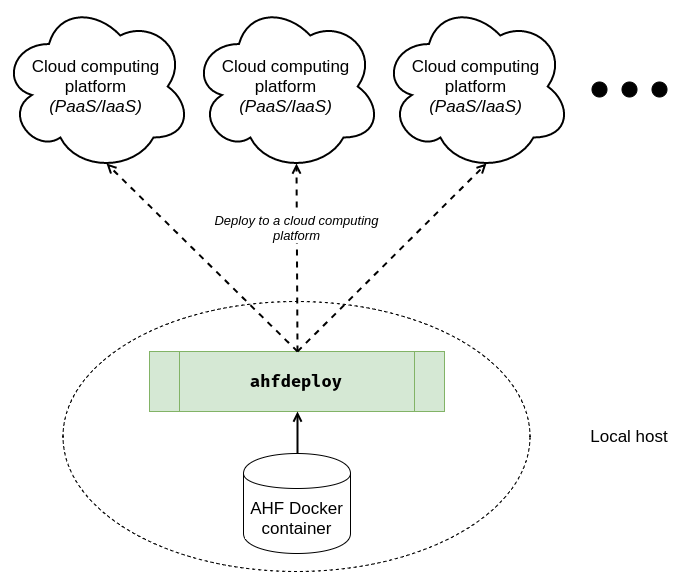
\includegraphics[keepaspectratio, width=14cm]{ahf_overview.png}
    \caption{Overview of the project with \texttt{ahfdeploy} highlighted in green.}
    \label{fig:overview}
\end{figure}

Figure \ref{fig:overview} shows an overview over an AHF docker container and some global cloud service providers. The green part, \texttt{ahfdeploy}, is supposed to deploy the docker onto one of these cloud services. \texttt{ahfdeploy} is also the part that we focus on in this project. It is our assignment to implement the behaviour and functionality.

Below is an example of usage of a potential CLI:
\bigskip
\midrule
\begin{minted}{bash}
  user@mainframe $ ahfdeploy -container ./AHF-Dockerfile \
                             -provider aws \
                             -token MTUxMTk1NTY0NHxEdi1CQkFFQ180S
  Deploying to Amazon AWS...
  Done!

  The instance is located at: proto://198.51.100.163:8471
  user@mainframe $ 
\end{minted}
\bigskip
\midrule

This is an desirable way of usage as for now that we will aim towards at the start of the project. The syntax may vary, but usage should be as easy as possible and target the above example. 

\subsection{Modules}
\begin{figure}[H]
    \centering
    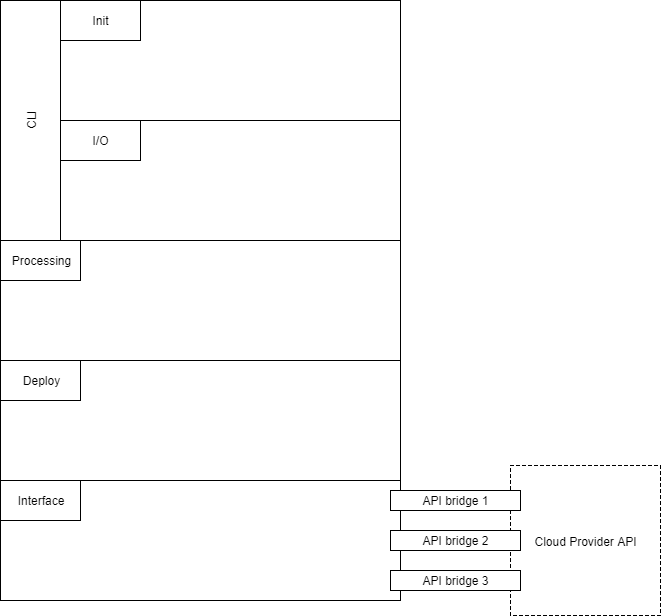
\includegraphics[keepaspectratio, width=14cm]{module.png}
    \caption{Module diagram of \texttt{ahfdeploy}s core.}
    \label{fig:module}
\end{figure}

Illustrated in figure \ref{fig:module} is a more detailed view of the different modules \texttt{ahfdeploy} will be built on. While showing what \texttt{ahfdeploy} will be doing in figure \ref{fig:overview}, figure \ref{fig:module} shows how \texttt{ahfdeploy} is going to be built from a modules point of view. 

The user of \texttt{ahfdeploy} will be communicating with the program via the CLI module. Closely related to the CLI are the Initialization and I/O modules. The Initialization module is intended to be called via a specific CLI command where the user can store credentials and other global settings. At this point we are not sure what kind of data we are going to deal with here, but we are convinced we well need this module. As of now, we are seeing the module taking an file as an argument and setting global settings according to the file.

I/O module will be responsible of loading the data given by the CLI command arguments, such as the container it self. This module will most likely consist of functions that read files. 

Before deploying the container to the cloud, we maybe need to make adjustment to the package that we send to the cloud provider. This module will be responsible for those classes and functions. Exact functions and classes may raise throughout the development process.

Deploying the module will be done via an interface that communicates with the specific cloud provider API. Since we are aiming for an general deploying application that shall support many different providers, the interface will need to link the container for the several API bridges for the specific provider API.
\newpage
\section{Implementation}

\subsection{Working model}
% Övergripande beskrivning av hur SCRUM tillämpats

\subsubsection{Reflections on implementation}
% Beskrivning och reflektioner utifrån projektets medlemmar, roller, möten, leveranser, planering av uppgifter, arbete med projektägareoch hantering av projektvariablerna omfattning och kvalité, kopplat till arbetsmodell

\paragraph*{Edvin Sladic}
\paragraph*{Olof Enekvist}
\paragraph*{Niclas Vretborn}
\paragraph*{Robin Persson}
\paragraph*{Ridge Petterson}
\paragraph*{William Wennerström}

\newpage
\section{Results}

\subsection{Delivery}%?

\subsection{Testing}

\subsubsection{Strategy for testing}
The project will use a mix of different testing strategies, both manual and automatic methods.

\paragraph*{Change impact analysis}
During a project development life-cycle a simple thing as a different external package version can break the application, so-called "dependency hell" in everyday speech. To ensure that only the currently supported versions for each dependency is used a package manager will enforces the correct version. In this case the Go \emph{official experiment} package manager \emph{dep} (\url{https://github.com/golang/dep}) is used to lock each package version.

\paragraph*{Traceability}
For getting a quick overview over each dependency, both internally and externally, without looking inside the code base a traceability matrix is used. Internal dependencies are packages that exist in the code base, while external are third party dependencies. Every new baseline that is of significant change should be documented together with a matrix. In this case a new baseline denotes a new major version.

\paragraph*{Quality risk analysis}
A high probability of risk events occurring and their impact will be mitigated by using stand up meetings. During these meetings each individual will tell the team what they have done during the last week and what they will focus on the next coming week. If a team member feels that something can impact their work, they should inform and discuss together to minimize the likelihood of a risk event.

\paragraph*{Cross-functional testing}
As the development team is small, all team members can be given different areas in the project to handle. Therefore everyone will together form a cross-functional team that either during the stand up meetings or through a pull request review process can give their opinion or block the change altogether. This is to asses if what is being built is actually useful.

\subsubsection{Regression risks} 
As parts of our system is developed and expanding, the risk for bugs increase. While creating the Module diagram (figure~\ref{fig:module}), several regression risks came to the targeted solution. 
\begin{itemize}  
\item Unmasked regression - A change unmask a bug that did not exist before.
\begin{itemize}
    \item Running the CLI on one machine, with a certain operating system, may work properly. However running the same CLI on another operating system may introduce a bug.
    \item Communication between the interface and the cloud provider API could introduce unmasked regressions. It could work with a certain provider, but when changing to another, bugs may appear.
\end{itemize}
\item Local regression - A change introduces a bug inside a module or component.
\begin{itemize}
    \item Expanding method functionality always have a risk of causing local regressions. I.e a \texttt{WriteToFile} method is extended with JIS encoding, however certain characters are written strangely or not at all.
\end{itemize}
\item Remote regression - A change in one part of the program breaks another part.
\begin{itemize}
    \item Altering methods in the I/O module could create bugs in the Processing module.
    \item A change in the architecture of the Cloud Provider API could break code in several other modules.
\end{itemize}
\end{itemize}

\subsubsection{Regression testing}
The two main ways to make test cases within software development processes is to either do a test-driven development (TDD) or a behavior-driven development (BDD).

This project uses both strategies, where the TDD approach handles the internal testing of the code base. And BDD tests the external command line interface.

For running automated tests a \emph{Continuous Integration} (CI) environment is used. The CI runs all tests on each code push to make sure no undetected regressions are merged. The CI of our choice is \emph{Travis CI} (\url{https://travis-ci.com}). Because GitHub is used for development, the CI will be integrated in the review process of a \emph{merge request} (or \emph{pull request}). GitHub will block each request that has failed tests until either they are fixed, or a reviewer overrides and merges any way.

The test driven development (TDD) is a development process that runs on very specific test cases in short development cycles. The whole development process revolves around making tests that are not based on previous tests but should work with the other tests. Then from the test you write your code, to then run more tests so you can edit the code where it is needed. Then repeat the process.

The benefits in running TDD is that we're testing the code as we go along so it wont be as many errors and regressions as it might otherwise normally be. Though it will require a lot more work and fall short on full system tests since you test each unit alone and not everything together.

Our language of choice, Go, has built-in support for unit testing code, both in a black box (package-wise, only public methods) and white box manner (accessing private methods). Currently the black box method is used, together with a coverage tool we ensure that all code (even private methods) are covered.

All unit tests should cover all lines in our code, so all cases are covered. A code coverage utility, \emph{Cover} (\url{https://golang.org/cmd/cover/}), is also bundled together with the Go toolchain. This tool is run on each code push and gives a good indication of our current code quality.

Behavioral driven development (BDD) is a development process that relates with TDD. It takes the principles and general techniques from it's predecessor and combines it with domain driven and object oriented analysis and design. 

When running with BDD tests, the main focus should be to learn and understand what is desired and expected behavior. The idea is to start with writing a test which defines a feature. Run this test, in other words let it fail. Then implement a unit that full fills the test. If the test passes, the feature is done. All tests should be defined in such a way that they describe the desired behavior.

One way to make BDD more effective is to use specialized software tools that automates the running of tests, and in some cases also automatically generates template code for new units.

Behavioral test units can also be run in the same manner inside a CI environment in our case. With a framework such as \emph{Ginkgo} (\url{https://onsi.github.io/ginkgo/}) the process can be automated.

\newpage
\subsubsection{Development description}
% Beskrivning av ”story/requirement” för utveckling av stöd för automatiserad (”unit testing”) 
% enhetstestning (”technology facing”) respektive automatiserad systemtestning (”business 
% facing”), dvs. totalt två ”stories”
Below are formal descriptions of unit tests that tries all different inputs and what the expected outputs are.

\begin{center}
\large{\underline{\textbf{1. Unit test:} \texttt{ReadContainer}}}
\vspace{-10px}
\end{center}
\begin{table}[H]
\centering
\begin{tabular}{ll}
\textbf{Signature}   & \mint{go}|func ReadContainer(*io.Reader, Checksum) (*Container, error)| \\
\textbf{Description} & Read and compare checksum container data before packaging and deployment.
\end{tabular}
\end{table}
\vspace{-12px}
\begin{table}[H]
\centering
\begin{tabular}{|p{8cm}|p{8cm}|}
\hline
\textbf{Input} & \textbf{Output} \\ \hline
A \textcolor{green}{valid reader} and \textcolor{green}{correct checksum}. & A \textcolor{green}{valid container} with \textcolor{green}{no error}. \\ \hline
An \textcolor{red}{invalid reader} and \textcolor{green}{correct checksum}. & \textcolor{red}{No container} with \textcolor{red}{invalid reader error}. \\ \hline
A \textcolor{green}{valid reader} and \textcolor{red}{incorrect checksum}. & \textcolor{red}{No container} with \textcolor{red}{incorrect checksum error}. \\ \hline
An \textcolor{red}{invalid reader} and \textcolor{red}{incorrect checksum}. & \textcolor{red}{No container} with \textcolor{red}{invalid reader error}. \\ \hline
\end{tabular}
\end{table}

Below follows formal descriptions of behavioral tests that can be integrated into one of the automated tools previously mentioned.

\definecolor{green}{RGB}{0, 100, 0}
\definecolor{red}{RGB}{100, 0, 0}
\begin{center}
\large{\underline{\textbf{2. Behavioral test:} \texttt{init}}}
\vspace{-10px}
\end{center}
\begin{table}[H]
\centering
\begin{tabular}{ll}
\textbf{Story}   & \texttt{Initialization of cloud deployment} \\
\textbf{As an} & AHF user. \\
\textbf{In order to} & The software to be effective. \\
\textbf{I want to} & Save my credentials so I don't have to repeat them when deploying containers to a \\& cloud service.
\end{tabular}
\end{table}
\vspace{-12px}
\begin{table}[H]
\centering
\begin{tabular}{|p{8cm}|p{8cm}|}
\hline
\textbf{Input} & \textbf{Output} \\ \hline
Credentials are entered and cloud API \textcolor{green}{handshakes}. & CLI informs of \textcolor{green}{connection test success} to cloud and credentials are \textcolor{green}{saved to a file}. \\ \hline
Credentials are entered but the cloud API \textcolor{red}{does not handshake}. & CLI informs of \textcolor{red}{connection test failed}, echoes the error message returned by the API, 
logs all data communication between software and cloud API in a session error log and credentials are \textcolor{red}{not saved to a file}. \\ \hline
\end{tabular}
\end{table}

\subsection{Ethics}

\subsection{Continuation}

\newpage
\section{Conclusion}

\newpage
\section{References}

\newpage
\section{Annex A - Instructions}



\end{document}